\begin{mainquestion}{pmosiv}{PMOS I-V Family Plot}

Use MATLAB, Excel, or some equivalent graphing software to plot the family of $i_{D}$ versus $v_{DS}$ curves for a PMOS transistor with $k_{p} = 1.5\ \frac{\text{mA}}{V^{2}}$ and $V_{tp} = -\qty{0.4}{\volt}$. Plot a curve for each integer voltage of $v_{GS}$ from 0 V to $-5$ V, and consider $-5 \leq v_{DS} \leq 0$. Make sure to denote the three operating regions on the plot and mark the boundary between triode and saturation with a dotted line as we did in the NMOS case on slide 13 from Lecture Notes \#6. You may assume $\lambda = 0$. Don't forget that we use the convention that $i_{D}$ is positive when flowing from source to drain in PMOS as well as in NMOS when flowing from drain to source.

\begin{partquestion}{plotfamily}{Plot the desired PMOS I-V family and provide the script.}
\begin{answer}
Here is a MATLAB script which generates the desired results:

\begin{verbatim}
kp=1.5;         % given parameters
Vtp=-0.4;
vDS=-5:.01:0;   % range of interest for vDS
for vGS=-5:0
    if vGS>Vtp  % check to see if in cutoff
        iD=zeros(size(vDS));
    else % not in cutoff, find vDS range that is in triode or in saturation and calculate current
        % triode case
        iD(find(vDS > vGS-Vtp))=kp*((-vGS+Vtp)*(-vDS(find(vDS > vGS-Vtp)))-0.5*vDS(find(vDS > vGS-Vtp)).^2);
        % saturation case
        iD(find(vDS <= vGS-Vtp))=0.5*kp*(-vGS+Vtp)^2;
    end
    plot(vDS,iD);   % plot curve for one value of vGS
    text(-5,iD(1)-.2+.9*(vGS~=0),strcat('{\itv_{GS}} = ',num2str(vGS))) % label curve
    hold on;
end
plot(vDS,0.5*kp*vDS.^2,'k--') % plot boundary between saturation and triode
xlabel('{\itv_{DS}} (V)');          % axis labels
ylabel('{\iti_D} (mA)',Rotation=0);
text(-4,7,'Saturation');            % graph annotations
text(-2.5,7,'Triode');
text(-4,0,'Cutoff');
hold off;
\end{verbatim}

This results in the following graph output:

\begin{center}
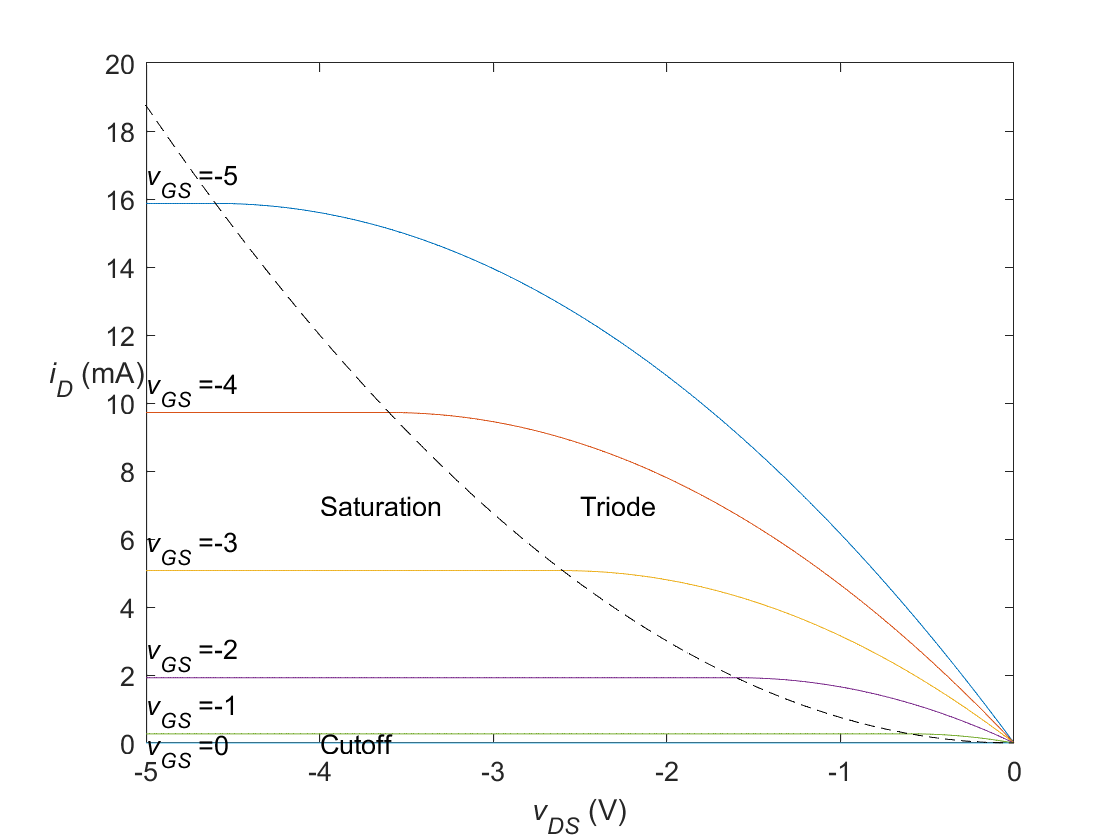
\includegraphics[width=5in]{plot.png}
\end{center}
\end{answer}
\end{partquestion}

\end{mainquestion}
